\chapter{Maximum-Likelihood and Bayesian Parameter Estimation}
Until now we have seen cases in which the parameters of the distributions were known. Now we'll look on how to estimate also this data. \newline
Let's suppose to have data sampled from a probability distribution $p(x,y)$, but while the form of the distribution is known, the parameters of such are not.  Let's suppose also to have a training set $\mathcal{D}=\{(x_1, y_1),\hdots,(x_m,y_m)\}$ of examples sampled independently and identically distributed\footnote{\textit{Independent}: each example is sampled independently from the others; \textit{identically distributed}: all examples are sampled from the same distribution.} according to $p(x,y)$. The goal is to estimate the unkown parameters of $p$ from the training data $\mathcal{D}$. \newline
Let's consider a multiclass classification problem: the training set can be divided into $\mathcal{D}_1,\hdots, \mathcal{D}_c$ subsets, one for each class. Mind that each subset contains iid examples for target class $y_i$: $\mathcal{D}_i=\{\vect{x}_1,\hdots,\vect{x}_n\}$. \newline
If the goal is to compute the probability of a class for a new example $\vect{x}$, then we can compute the probability of a class given the new example and all the dataset as described by Bayes rule, Definition~\ref{def:BayesRule}:
\begin{center}
	$\displaystyle P(y_i\vert\vect{x},\mathcal{D})=\cfrac{p(\vect{x}\vert y_i,\mathcal{D})p(y_i\vert\mathcal{D})}{p(\vect{x}\vert\mathcal{D})}$
\end{center}
To really get the class of the new example we are going to compute the probability for all possible classes and then maximize over it. \newline
Since $\vect{x}$ will be in a class $y_i$, it's safe to assume that it will be independent of $D_j, i\neq j$. It's possible to notice that the term $p(y_i\vert D)$ is the probability of finding a class inside the dataset, for example if the dataset contained students, and the class were to be Italian students, so it simply is:
\begin{center}
	$\displaystyle p(y_i\vert \mathcal{D})=\frac{\abs{D_i}}{\abs{D}}$
\end{center}
As for the denominator, it's possible to marginalize (Sum rule~\ref{def:SumRule}) $p(\vect{x}\vert y_i,\mathcal{D}_i)p(y_i\vert \mathcal{D})$ over all possible classes:
\begin{center}
	$\displaystyle p(\vect{x}\vert \mathcal{D})=\Sum_{y_i}p(\vect{x}\vert y_i,\mathcal{D}_i)p(y_i\vert \mathcal{D})$
\end{center}
The idea of this step is that $y_i$ does not depend on all $\mathcal{D}$, but only on $\mathcal{D}_i$.\newline
The goal is to estimate \textit{class-dependent} parameters $\theta_i$ for $\displaystyle p(\vect{x}\vert y_i,\mathcal{D}_i)$. There are two ways to solve this problem:
\begin{itemize}
	\item \textbf{Bayesian estimation}: assumes that parameters $\theta_i$ are random variables with some known prior distribution. Once the example has been observed, the probability becomes a posterior distribution. Predictions for new examples are obtained integrating over all possible values for the parameters:
		\begin{center}
			$\displaystyle p(\vect{x}\vert y_i,\mathcal{D}_i)=\int_{\theta_i}p(\vect{x},\theta_i\vert y_i,\mathcal{D}_i)d\theta_i$
		\end{center}
	\item \textbf{Maximum likelihood}: The parameters are computed as those maximising the probability of the observed examples $\mathcal{D}_i$, that is the training set for the class. For such reason they can be used to compute the probability for the new examples:
		\begin{center}
			$\displaystyle p(\vect{x}\vert y_i,\mathcal{D}_i)\approx p(\vect{x}\vert\theta_i)$
		\end{center}
\end{itemize}
%
%
%
\section{Maximum likelihood}
\label{sec:MaximumLikelihood}
%TODO Can I remove these?
\newcommand{\maxl}{0}{maximum likelihood}
\newcommand{\Maxl}{0}{Maximum likelihood}
If we can assume a prior distribution for the parameters $p(\theta_i)$, then maximum likelihood becomes maximum a-posteriori estimation and can be summarized as:
\begin{center}
	$\displaystyle \theta^*_i=\argmax{\theta_i}p(\theta_i\vert\mathcal{D}_i,y_i)=\argmax{\theta_i}p(\mathcal{D}_i,y_i\vert \theta_i)p(\theta_i)$
\end{center}
If a priori distribution is not available, then the solution is indeed maximum likelihood, that is maximizing the likelihood of the parameters with respect to the training samples:
\begin{center}
	$\displaystyle \theta_i^*=\argmax{\theta_i}p(\mathcal{D}_i,y_i\vert\theta_i)$
\end{center}
From now on, for simplicity, since each class $y_i$ is trated independentely, we'll write $y_i, \mathcal{D_i}$ as simply $\mathcal{D}$.\newline
Given a training dataset $\mathcal{D}=\{\vect{x}_1,\hdots,\vect{x}_n\}$ of iid examples for the target class $y$, assumed that the parameter vector $\vect{\theta}$ has a fixed but unknown value, we estimate such value by maximizing its likelihood with respect to the training data:
\begin{center}
	$\displaystyle \theta^*=\argmax{\vect{\theta}}p(\mathcal{D}\vert\vect{\theta})$
\end{center}
Since the examples are iid, the joint probability over $\mathcal{D}$ can be decomposed into a product:
\begin{center}
	$\displaystyle \theta^*=\argmax{\vect{\theta}}\Prod_{j=1}^np(\vect{x}_j\vert\vect{\theta})$
\end{center}
Moreover we don't generally like products, and since the goal is to maximize, it is possible to maximize over the logarithm of the product which equals to the sum of the logarithms. This is possible because the logarithm function is monotonic:
\begin{center}
	$\displaystyle \theta^*=\argmax{\vect{\theta}}\ln{p(\mathcal{D}\vert\vect{\theta})}=\argmax{\vect{\theta}}\ln{\Prod_{j=1}^np(\vect{x}_j\vert\vect{\theta})}$\\
	\vspace{0.3cm}
	$\displaystyle \theta^*=\argmax{\vect{\theta}}\Sum_{j=1}^n\ln{p(\vect{x}_j\vert\vect{\theta})}$\\
\end{center}
This is also called \textit{maximizing the log-likelihood}. \newline
The maxima can be obtained zeroing the gradient with respect to $\vect{\theta}$:
\begin{center}
	$\displaystyle \nabla_{\vect{\theta}}=\Sum_{j=1}^n\ln{p(\vect{x}_j\vert\vect{\theta})}=\vect{0}$
\end{center}
Since points zeroing the gradient can be local or global maxima.\newline
%
%
\subsection{Example -- Univariate Gaussian}
Let's consider a Gaussian distribution (Equation~\ref{eq:Gaussian}) with unknown $\mu$ and $\sigma^2$, then the log-likelihood $\mathcal{L}$ is:
\begin{center}
\begin{tabular}{rl}
	$\displaystyle \mathcal{L}=$&$\displaystyle\Sum_{j=1}^n\ln{\cfrac{1}{\sqrt{2\pi\sigma}}~e^{-\cfrac{(x_j-\mu)^2}{2\sigma^2}}}$\\
	$=$&$\displaystyle \Sum_{j=1}^n-\cfrac{1}{2\sigma^2}(x_j-\mu)^2-\frac{1}{2}\ln{2\pi\sigma^2}$
\end{tabular}
\end{center}
Now let's do the gradient with respect to $\theta$, that is derive first for $\mu$ and then for $\sigma^2$:
\[\nabla_\theta=
\begin{cases}
	\cfrac{\partial\mathcal{L}}{\partial\mu}\\
	\cfrac{\partial\mathcal{L}}{\partial\sigma^2}\\
\end{cases}
\]
Let's do the one respect to $\mu$ first:
\begin{center}
\begin{tabular}{rl}
	$\cfrac{\partial\mathcal{L}}{\partial\mu}=$&$\displaystyle -\Sum_{j=1}^n \cfrac{1}{2\sigma^2}(2\mu-2x_j)+0$\\
	$=$&$\displaystyle \Sum_{j=1}^n\cfrac{1}{\sigma^2}(x_j-\mu)$
\end{tabular}
\end{center}
Let's then do the one respect to $\sigma^2$:
\begin{center}
\begin{tabular}{rl}
	$\cfrac{\partial\mathcal{L}}{\partial\sigma^2}=$&$\displaystyle -\Sum_{j=1}^n \cfrac{1}{2\sigma^2}(2\mu-2x_j)-\cfrac{1}{2}\ln{2\pi\sigma^2}$\\
	$=$&$\displaystyle -\Sum_{j=1}^n\left[\cfrac{1}{2}(x_j-\mu)^2\cfrac{\partial}{\partial \sigma^2}\cfrac{1}{\sigma^2}\right]-\cfrac{n}{2}\cfrac{\partial}{\partial\sigma^2}\ln{2\pi\sigma^2}$\\
	$=$&$\displaystyle -\cfrac{n}{2}2\pi\cfrac{1}{2\pi\sigma^2}-\Sum_{j=1}^n\cfrac{(x_j-\mu)^2}{2}(-1)\cfrac{1}{\sigma^4}$\\
	$=$&$\displaystyle -\cfrac{n}{2\sigma^2}+\Sum_{j=1}^n\cfrac{(x_j-\mu)^2}{2\sigma^4}$
\end{tabular}
\end{center}
The gradient with respect to the parameters is:
\[\nabla_\theta=
\begin{cases}
	\cfrac{\partial\mathcal{L}}{\partial\mu}=\Sum_{j=1}^n\cfrac{1}{\sigma^2}(x_j-\mu)\\
	\cfrac{\partial\mathcal{L}}{\partial\sigma^2}=-\cfrac{n}{2\sigma^2}+\Sum_{j=1}^n\cfrac{(x_j-\mu)^2}{2\sigma^4}\\
\end{cases}
\]
Now we need to zero the gradient. First for $\mu$:
\begin{center}
	$\displaystyle \Sum_{j=1}^n\cfrac{1}{\sigma^2}(x_j-\mu)=0$\\
	$\displaystyle \Sum_{j=1}^n(x_j-\mu)=0$\\
	$\displaystyle \Sum_{j=1}^nx_j-\Sum_{j=1}^n\mu=0$\\
	$\displaystyle \Sum_{j=1}^nx_j=\Sum_{j=1}^n\mu$\\
	$\displaystyle \Sum_{j=1}^nx_j=n\mu$	\\
	$\displaystyle \mu=\cfrac{1}{n}\Sum_{j=1}^nx_j$	
\end{center}
Now let's do the one for $\sigma^2$:
\begin{center}
	$\displaystyle -\cfrac{n}{2\sigma^2}+\Sum_{j=1}^n\cfrac{(x_j-\mu)^2}{2\sigma^4}=0$\\
	$\displaystyle \Sum_{j=1}^n\cfrac{(x_j-\mu)^2}{2\sigma^4}=\cfrac{n}{2\sigma^2}$\\
	$\displaystyle \cfrac{1}{2\sigma^4}\Sum_{j=1}^n(x_j-\mu)^2=\cfrac{n}{2\sigma^2}$\\
	$\displaystyle \cfrac{1}{\sigma^2}\Sum_{j=1}^n(x_j-\mu)^2=n$\\
	$\displaystyle \sigma^2=\cfrac{1}{n}\Sum_{j=1}^n(x_j-\mu)^2$\\
\end{center}
So the maximum-likelihood estimates are:
\begin{center}
	$\displaystyle \mu=\cfrac{1}{n}\Sum_{j=1}^nx_j$\\
	\vspace{0.3cm}
	$\displaystyle \sigma^2=\cfrac{1}{n}\Sum_{j=1}^n(x_j-\mu)^2$
\end{center}
\subsection{Example -- Multivariate Gaussian}
Let's recall the multivariate distribution (Equation~\ref{eq:MultivariateGaussian}):
\begin{center}
	$\displaystyle p(\vect{x};\mu,\Sigma)=\cfrac{1}{(2\pi)^{\myfrac{d}{2}}\abs{\Sigma}^{\myfrac{1}{2}}}e^{-\frac{1}{2}(\vect{x}-\vect{\mu})^T\Sigma^{-1}(\vect{x}-\vect{\mu})}$
\end{center}
The log-likelihood is:
\begin{center}
	$\displaystyle \Sum_{j=1}^n-\frac{1}{2}(\vect{x}_j-\vect{\mu})^T\Sigma^{-1}(\vect{x}_j-\vect{\mu})-\frac{1}{2}\ln{(2\pi)^d\abs{\Sigma}}$
\end{center}
And the maximum -likelihood estimates are:
\begin{center}
	$\displaystyle \mu=\frac{1}{n}\Sum_{j=1}^n\vect{x}_j$\\
	$\displaystyle \Sigma=\frac{1}{n}\Sum_{j=1}^n(\vect{x}_j\vect{\mu})(\vect{x}_j-\vect{\mu})^T$
\end{center}
\vspace{1cm}
It's possible to notice then, that for Gaussian distributions, the parameters are simply their empirical estimates over the sample:
\begin{itemize}
	\item Gaussian mean is the sample mean;
	\item Gaussian covariance matrix is the mean of the sample covariances.
\end{itemize}
%
%
%
\section{Bayesian estimation}
\label{sec:BayesEstimation}
\newcommand{\best}[1]{beasyan estimation~}
\newcommand{\Best}[1]{beasyan estimation~}
%TODO change theta to \vect{\theta} in all equations before
Let's assume that parameters $\theta_i$ are \textit{random variables} with some known \textit{prior} distribution. \newline
Predictions for new examples are obtained integrating over all possible values for the parameters:
\begin{center}
	$\displaystyle p(\vect{x}\vert y_i, \mathcal{D}_i)=\int_{\vect{\theta}_i}p(\vect{x},\vect{\theta}_i\vert y_i,\mathcal{D}_i)d\vect{\theta}_i$
\end{center}
Probability of $\vect{x}$ given each class $y_i$ is independent of the other classes $y_i$, for simplicity we can again write:
\begin{center}
	$\displaystyle p(\vect{x}\vert y_i, \mathcal{D}_i)\rightarrow p(\vect{x}\vert\mathcal{D})=\int_{\vect{\theta}}p(\vect{x},\vect{\theta}\vert \mathcal{D})d\vect{\theta}$
\end{center}
Where $\mathcal{D}$ is a dataset for a certain class $y$, and $\vect{\theta}$ the parameters of the distribution. \newline
%TODO prova a vedere se Marco capisce il passaggio intermedio 😩😩😩😩
\begin{equation}
	p(\vect{x}\vert\mathcal{D})=\int_{\vect{\theta}}p(\vect{x},\vect{\theta}\vert\mathcal{D})d\vect{\theta}=\int_{\vect{\theta}} p(x\vert\vect{\theta}, D)p(\vect{\theta}\vert D)d\vect{\theta}=\int_{\vect{\theta}}p(\vect{x}\vert\vect{\theta})p(\vect{\theta}\vert\mathcal{D})d\vect{\theta}
	\label{eq:classConditionalDensity}
\end{equation}
Where $p(\vect{x}\vert\mathcal{D})$ can be easily computed since we have both form and parameters of the distribution, e.g., if it were a gaussian the form is Equation~\ref{eq:Gaussian}, while the parameters are $\mu$ and $\sigma^2$. \newline
Since our goal is to estimate the parameters' posterior density given a training set $p(\vect{\theta}\vert\mathcal{D})$ by using Bayes rule (Definition~\ref{def:BayesRule}), then we can write:
\begin{center}
	$\displaystyle p(\vect{\theta}\vert \mathcal{D})=\frac{p(\mathcal{D}\vert\vect{\theta})p(\vect{\theta})}{p(\mathcal{D})}=\frac{\left(\Prod_{j=i}^n(P(\vect{x}_i\vert \vect{\vect{\theta}})\right)P(\vect{\theta})}{P(\mathcal{D})}$
\end{center}
$P(\mathcal{D}\vert \vect{\theta})$ is the likelihood probability that has been used also in the maximum likelihood method. In this case though, the parameters are weighted with respect to their probability avoiding overfitting which is a problem of maximum likelihood.\newline
Mind that $P(\mathcal{D})$ is a constant independent of $\theta$, hence it will have no influence in the final Bayesian decision, therefore it can be neglected. \newline
At last, if final probability is needed, then $P(\mathcal{D})$ is computable via:
\begin{center}
	$\displaystyle p(\mathcal{D})=\int_{\vect{\theta}}p(\mathcal{D}\vert\vect{\theta})p(\vect{\theta})d\vect{\theta}$
\end{center} 
%
%
\subsection{Example -- Univariate Normal, unknown $\mu$, known $\sigma^2$}
Example are drawn from a normal distribution, hence:
\begin{center}
	$\displaystyle p(\vect{x}\vert\vect{\theta})=p(x\vert\mu)\sim N(\mu, \sigma^2)$
\end{center}
Moreover the Gaussian mean distribution is itself a normal distribution:
\begin{center}
	$\displaystyle P(\mu)\sim N(\mu_0, \sigma_0^2)$
\end{center}
So the distribution of the parameter's posterior distribution can be computed as:
\begin{center}
	$\displaystyle p(\mu\vert\mathcal{D})=\cfrac{p(\mathcal{D}\vert\mu)p(\mu)}{p(\mathcal{D})}=\cfrac{1}{p(\mathcal{D})}\left(\Prod_{j=1}^np(x_j\vert\mu)\right)p(\mu)$
\end{center}
Where we said that $p(x_j\vert \mu)\sim N(\mu,\sigma^2)$ and $p(\mu)\sim N(\mu_0,\sigma_0^2)$:
\[
	p(\mu\vert\mathcal{D})=\cfrac{1}{p(\mathcal{D})}\left(\Prod_{j=1}^n
	\underbrace{\cfrac{1}{\sigma\sqrt{2\pi}}e^{-\cfrac{(x_j-\mu)^2}{2\sigma^2}}\rule[-12pt]{0pt}{5pt}}_{\mbox{$p(x_j\vert\mu)$}}\right)
	\underbrace{\cfrac{1}{\sigma_0\sqrt{2\pi}}e^{-\cfrac{(\mu-\mu_0)^2}{2\sigma_0^2}}\rule[-12pt]{0pt}{5pt}}_{\mbox{$p(\mu)$}}
\]
Since $p(\mathcal{D})$ is constant, it can be moved out of the product, and we'll call it $\alpha=\myfrac{1}{p(\mathcal{D})}$:
\[
	p(\mu\vert\mathcal{D})=\alpha \Prod_{j=1}^n \cfrac{1}{\sigma\sqrt{2\pi}}e^{-\cfrac{(x_j-\mu)^2}{2\sigma^2}}\cfrac{1}{\sigma_0\sqrt{2\pi}}e^{-\cfrac{(\mu-\mu_0)^2}{2\sigma_0^2}}
\]
Now we could use the exponentiation's properties:
\[e^x\times e^y=e^{x+y}\]
\[\Prod_i e^{x_i}=e^{\Sigma_i x_i}\]
Before though, the constant parts could be moved outside the product and we'll call the new constant part outside the product as $\alpha'$:
\[
	p(\mu\vert\mathcal{D})=\alpha \left(\cfrac{1}{2\sigma\sigma_0\pi}\right)^n\left(\Prod_{j=1}^n \exp{-\cfrac{(x_j-\mu)^2}{2\sigma^2}}\right)\exp{-\cfrac{(\mu-\mu_0)^2}{2\sigma_0^2}}
\]
\[
	p(\mu\vert\mathcal{D})=\alpha' \exp{\Sum_{j=1}^n-\frac{(x_j-\mu)^2}{2\sigma^2}}\exp {-\cfrac{(\mu-\mu_0)^2}{2\sigma_0^2}}
\]
\[
	p(\mu\vert\mathcal{D})=\alpha' \exp{\frac{1}{2}\left(\Sum_{j=1}^n\frac{(x_j-\mu)^2}{\sigma^2} +\cfrac{(\mu-\mu_0)^2}{\sigma_0^2}\right)}
\]
Let's now focus only on the exponent\footnote{$(x_j-\mu)^2=(\mu-x_j)^2$.}:
\[
	-\cfrac{1}{2}\left(\Sum_{j=1}^n\cfrac{(\mu-x_j)^2}{\sigma^2}+\cfrac{(\mu-\mu_0)^2}{\sigma_0^2}\right)
\]
Now it's possible to expand the exponentials:
\[
	-\cfrac{1}{2}\left(\Sum_{j=1}^n\cfrac{\mu^2+x_j^2-2\mu x_j}{\sigma^2}+\cfrac{\mu^2+\mu_0^2-2\mu\mu_0}{\sigma_0^2}\right)
\]
And move the constant term wrt to the sum outside the sum:
\[
	-\cfrac{1}{2}\left(\cfrac{n\mu^2}{\sigma^2}+\cfrac{1}{\sigma^2}\Sum_{j=1}^nx_j^2-\cfrac{1}{\sigma^2}\Sum_{j=1}^n2\mu x_j+\cfrac{\mu^2}{\sigma^2}+\cfrac{\mu_0^2}{\sigma^2}-\cfrac{2\mu\mu_0}{\sigma_0^2}\right)
\]
First of all let's group the common terms:
\[
	-\cfrac{1}{2}\left(\mu^2\left(\cfrac{n}{\sigma^2}+\cfrac{1}{\sigma^2}\right)+\cfrac{\mu_0^2}{\sigma^2}+\cfrac{1}{\sigma^2}\Sum_{j=1}^nx_j^2-2\mu\left(\cfrac{1}{\sigma^2}\Sum_{j=1}^n x_j-\cfrac{\mu_0}{\sigma_0^2}\right)\right)
\]
Let's now consider all the equation obtained:
\[
	p(\mu\vert\mathcal{D})=\alpha' \exp{-\cfrac{1}{2}\left(\mu^2\left(\cfrac{n}{\sigma^2}+\cfrac{1}{\sigma^2}\right)+\cfrac{\mu_0^2}{\sigma^2}+\cfrac{1}{\sigma^2}\Sum_{j=1}^nx_j^2-2\mu\left(\cfrac{1}{\sigma^2}\Sum_{j=1}^n x_j-\cfrac{\mu_0}{\sigma_0^2}\right)\right)}
\]
Mind now that this is, by the exponentials properties, the same as:
\[
	p(\mu\vert\mathcal{D})=\alpha' \exp{-\cfrac{1}{2}\left(\mu^2\left(\cfrac{n}{\sigma^2}+\cfrac{1}{\sigma^2}\right)-2\mu\left(\cfrac{1}{\sigma^2}\Sum_{j=1}^n x_j-\cfrac{\mu_0}{\sigma_0^2}\right)\right)}\exp{+\cfrac{\mu_0^2}{\sigma^2}+\cfrac{1}{\sigma^2}\Sum_{j=1}^nx_j^2}
\]
Where the second exponential is actually not dependent on $\mu$, hence it can be moved insider $\alpha'$ which then becomes $\alpha''=\alpha'\times\exp{+\cfrac{\mu_0^2}{\sigma^2}+\cfrac{1}{\sigma^2}\Sum_{j=1}^nx_j^2}$:
\[
	p(\mu\vert\mathcal{D})=\alpha'' \exp{-\cfrac{1}{2}\left(\mu^2\left(\cfrac{n}{\sigma^2}+\cfrac{1}{\sigma^2}\right)-2\mu\left(\cfrac{1}{\sigma^2}\Sum_{j=1}^n x_j-\cfrac{\mu_0}{\sigma_0^2}\right)\right)}
\]
It's possible to notice that this posterior probability is quite similar with a normal, let's describe it as:
\begin{equation}
	p(\mu\vert \mathcal{D})=\cfrac{1}{\sqrt{2\pi}\sigma_n}\exp{-\frac{1}{2}\left(\frac{\mu-\mu_n}{\sigma_n}\right)^2}
	\label{eq:BayesianUnivariatePosteriorNormal}
\end{equation}
\[
	p(\mu\vert\mathcal{D})=\cfrac{1}{\sqrt{2\pi}\sigma_n}\exp{-\frac{1}{2}\left(\frac{\mu^2}{\sigma_n^2}+\frac{\mu_n^2}{\sigma_n^2}-\frac{2\mu\mu_n}{\sigma_n^2}\right)}
\]
\[
	p(\mu\vert\mathcal{D})=\cfrac{1}{\sqrt{2\pi}\sigma_n}\exp{\frac{\mu_n^2}{\sigma_n^2}}\exp{-\frac{1}{2}\left(\frac{\mu^2}{\sigma_n^2}-\frac{2\mu\mu_n}{\sigma_n^2}\right)}=\alpha'''\exp{-\frac{1}{2}\left(\frac{\mu^2}{\sigma_n^2}-\frac{2\mu\mu_n}{\sigma_n^2}\right)}
\]
By comparison with the equation obtained before it's possible to notice that:
\[
	\frac{1}{\sigma_n^2}=\frac{n}{\sigma^2}+\frac{1}{\sigma^2_0}\qquad \frac{\mu_n}{\sigma_n^2}=\frac{\mu_0}{\sigma_0^2}+\Sum_{j=1}^nx_j
\]
Let's first focus on the second equation. By multiplying and dividing for $n$ the sum, it's possible to obtain the sample mean $\widehat{\mu}_n$:
\[
	\frac{\mu_n}{\sigma_n^2}=\frac{\mu_0}{\sigma_0^2}+n\frac{1}{n}\Sum_{j=1}^nx_j=\frac{\mu_0}{\sigma_0^2}+n\widehat{\mu}_n
\]
Now let's solve for $\sigma_n$ first since $\mu_n$ depends on $\sigma_n$:
\[
	\frac{1}{\sigma^2_n}=\frac{n\sigma^2_0+\sigma^2}{\sigma^2\sigma_0^2}
\]
\[
	\sigma^2_n=\frac{\sigma^2\sigma_0^2}{n\sigma^2_0+\sigma^2}
\]
It's now possible to solve for $\mu_n$:
\[
	\mu_n=n\widehat{\mu}_n\sigma^2_n+\frac{\mu_0\sigma_n^2}{\sigma_0}
\]
\[
	\mu_n=n\widehat{\mu}_n\frac{\sigma^2\sigma_0^2}{n\sigma^2_0+\sigma^2}+\mu_0\frac{\sigma^2}{n\sigma^2_0+\sigma^2}
\]
Notice that the men $\mu_n$ is a linear combination of the prior $\mu_0$ and the sample mean $\widehat{\mu}_n$. If the number of samples increases, the sample mean starts to dominate over the prior mean and the variance decreases, making the distribution sharply peaked over its mean.
\begin{center}
	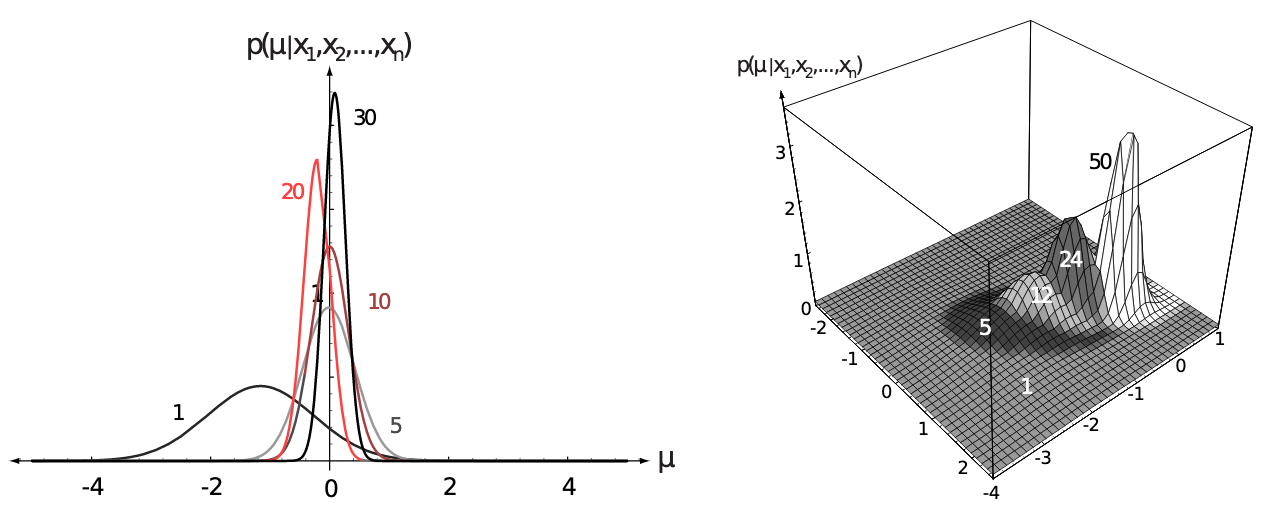
\includegraphics[width=\linewidth]{BayesianEstimationUnivariateExample1}
\end{center}
We stil haven't computed the class conditional density $p(x\vert\mathcal{D})$. Remember Equation~\ref{eq:classConditionalDensity}:
\[
	P(x\vert \mathcal{D})=\int_\mu P(x\vert \mu)P(\mu\vert \mathcal{D})\d\mu
\]
Since we said that $p(x\vert\mu)\sim N(\mu, \sigma^2)$, and from what was achieved in Equation~\ref{eq:BayesianUnivariatePosteriorNormal}, it's possible to write:
\[
	p(x\vert \mathcal{D})=\int_\mu N(\mu, \sigma^2)N(\mu_n, \sigma_n^2)d\mu
\]
\[
	p(x\vert \mathcal{D})=\int_\mu \cfrac{1}{\sqrt{2\pi}\sigma}\exp{-\frac{1}{2}\left(\frac{x-\mu}{\sigma}\right)^2} \cfrac{1}{\sqrt{2\pi}\sigma_n}\exp{-\frac{1}{2}\left(\frac{\mu-\mu_n}{\sigma_n}\right)^2} d\mu
\]
Let's now define $f(\sigma,\sigma_n)$:
\[
	f(\sigma,\sigma_n)=\int_\mu\exp{-\frac{1}{2}\frac{\sigma^2+\sigma_n^2}{\sigma^2\sigma^n}\left(\mu-\frac{\sigma_n^2x+\sigma^2\mu_n}{\sigma^2+\sigma_n^2} \right)^2}d\mu
\]
Then we could rewrite the previous probability as:
\[
	p(x\vert \mathcal{D})=\int_\mu \cfrac{1}{2\pi\sigma\sigma_n}
	\underbrace{\exp{-\frac{1}{2}\frac{(x-\mu_n)^2}{\sigma^2+\sigma_n^2}}\rule[-12pt]{0pt}{5pt}}_{\mbox{$\beta$}} 
	f(\sigma,\sigma_n)
\]
If we consider $p(x\vert\mathcal{D})$ as a function of $x$, then it is proportional to $\beta$ in the previous equation and hence $p(x\vert\mathcal{D})$ is normally distributed with mean $\mu_n$ and variance $\sigma^2+\sigma^2_n$:
\[
	p(x\vert\mathcal{D})\sim N(\mu_n,\sigma^2+\sigma^2_n)
\]
This means that the probability of $x$ given the dataset for the class is a Gaussian with mean equal to the posterior mean, and the variance equal to the sum of the known variance $(\sigma^2)$ and the additional variance $(\sigma^2)$due to the uncertainty of the mean.\newline
The same thing happens with the multivariate. Known that the examples are drawn from a multivariate and that also distribution of the mean for the multivariate is still a multivariate:
\[ p(\vect{x}\vert\vect{\mu})\sim N(\vect{\mu},\Sigma) \]
\[ p(\vect{\mu})\sim N(\vect{\mu}_0,\Sigma_0) \]
It's possible to obtain the posterior and the class-conditional distributions:
\[p(\vect{\mu}\vert\mathcal{D})\sim N(\vect{\mu}_n,\Sigma_n) \]
\[p(\vect{x}\vert\mathcal{D})\sim N(\vect{\mu}_n,\Sigma+\Sigma_n) \]
%
%
%
\section{Sufficient statics}
\begin{definition}[Statistic]
A function on a set of samples $\mathcal{D}$ is called statistic.
\end{definition}
One example of statistics is the mean. We'll use statistics to evaluate the forecast. \newline
\begin{definition}[Sufficient Statistic]
A statistic $\phi(\mathcal{D})$is said to be \textit{sufficient} for some parameters $\vect{\theta}$ if all we need to estimate the parameter is the statistic:
\[
	P(\mathcal{D}\vert\vect{s},\vect{\theta})=P(\mathcal{D}\vert\vect{s})
\]
\end{definition}
If $\vect{\theta}$ is a random variable, a sufficient statistic contains all relevant information $\mathcal{D}$ has for estimating it:
\[
	p(\vect{\theta}\vert\mathcal{D},\vect{ß})=\cfrac{p(\mathcal{D}\vert\theta,\vect{s})p(\vect{\theta}\vert\vect{s})}{p(\mathcal{D}\vert\vect{S})}=p(\vect{\theta}\vert\vect{s})
\]
For example if we consider the Gaussian, the sample mean was all one would need from the dataset, the exact values are meaningless. 
%
%
%
\data{10/10/2019}
\section{Conjugate}
\begin{definition}[Conjugate priors]
Given a likelihood function $p(x\vert\theta)$, given a prior distribution $p(\theta)$, $p(\theta)$ is said to be a conjugate prior for $p(x\vert\theta)$ if the posterior distribution $p(\theta\vert x)$ is the same family as the prior $p(\theta)$. 
\end{definition}
Over what was seen before about the univariate normal case, other examples are described in Table~\ref{tab:conjugateDistributions}. For example if we are trying to estimate samples taken from a Normal distribution ($p(x\vect\theta)\sim N(\mu, \sigma^2)$), and the modelled parameter is the mean, then the conjugate prior will still be a normal distribution. 
\begin{table}[htp]
	\centering
	\begin{tabular}{lll}
		Likelihood&Parameters&Conjugate Prior\\
		\hline
		Binomial&$p$ (probability)&Beta\\
		Multinomial&$\vect{p}$ (probability vector)&Dirichlet\\
		Normal&$\mu$ (mean)&Normal\\
		Multivariate Normal&$\vect{\mu}$ (mean vector)&Normal\\
	\end{tabular}
	\caption{Table showing the conjugate prior of a likelihood depending on the parameter.}
	\label{tab:conjugateDistributions}
\end{table}
%
%
\subsection{Bernoulli Distribution}
This distribution models boolean events, either they are "success", or they are "failure". The parameter $\theta$ of the Bernoulli is simply the probability of success. The mass function (which will be used in the likelihood) is:
\[
	P(x\vert\theta)=\theta^x(1-\theta)^{1-x}
\]
The conjugate prior is a Beta distribution:
\[
	P(\theta\vert\psi)=P(\theta\vert\alpha_h, \alpha_t)=\frac{\Gamma(\alpha)}{\Gamma(\alpha_h)\Gamma(\alpha_t)}\theta^{\alpha_h-1}(1-\theta)^{\alpha_t-1}
\]
%
%
\subsubsection{Example}
Let's consider a dataset made out of the results of tossing a coin:
\[
\mathcal{D}=\{H,H,T,T,T,H,H\}
\]
The parameter $\theta$ indicates the probability of tossing head. The likelihood function becomes:
\[
	p(\mathcal{D}\vert\theta)=\theta\cdot\theta\cdot(1-\theta)\cdot(1-\theta)\cdot(1-\theta)\cdot\theta\cdot\theta=\theta^h(1-\theta)^t
\]
First let's try to estimate $\theta$ via the maximum likelihood method seen in Section~\ref{sec:MaximumLikelihood}, that is basically deriving the log likelihood and seeing for what values it goes to zero.
\[
\cfrac{\partial}{\partial\theta}\ln{p(\mathcal{D}\vert\theta)}=0
\]
\[
\cfrac{\partial}{\partial\theta}\ln{\theta^h(1-\theta)^t}=0
\]
\[
\cfrac{\partial}{\partial\theta}h\ln{\theta}+t\ln{(1-\theta)}=0
\]
\[
h\frac{1}{\theta}+t\frac{1}{1-\theta}(-1)=0
\]
\[
\frac{h}{\theta}=\frac{t}{1-\theta}
\]
\[
h-\theta h=t\theta
\]
\[
\theta=\frac{h}{h+t}
\]
This tells us that $h,t$, that is the number of heads and tails in the dataset $\mathcal{D}$ respectively, are the sufficient parameters. This implies that for example we don't care about the order of the outcomes.\newline
Let's now try to estimate the value of the parameter $\theta$ by using the Bayesian estimation. We have seen in Section~\ref{sec:BayesEstimation} that the parameter posterior is proportional to:
\[
P(\theta\vert\mathcal{D},\psi)\propto P(\mathcal{D}\vert\theta)P(\theta\vert\psi)\propto\theta^h(1\-\theta)^t\theta^{\alpha_h-1}(1-\theta)^{\alpha_t-1}=\theta^{h+\alpha_h-1}(1-\theta)^{t+\alpha_t-1}
\]
That is the posterior is proportional to a Beta distribution with parameters $h+\alpha_h, t+\alpha_t$. \newline
The prediction for a new event it's basically the expected value of the posterior Beta: %TODO prova a vedere se per caso Marco sa perchè
\[
P(x\vert\mathcal{D})=\int P(x\vert\theta)P(\theta\vert\mathcal{D},\psi)d\theta
\]
The probability $P(x\vert\theta)$ is actually $\theta$ since the parameter represents the probability of success for an event. 
\[
P(x\vert\mathcal{D})=\int\theta P(\theta\vert\mathcal{D},\psi)d\theta
\]
Such integral is just the expected value of the Beta (Equation~\ref{eq:BetaStatistics}):
\[
P(x\vert\mathcal{D})=\text{E}_{P(\theta\vert\mathcal{D},\psi)}[\theta]=\cfrac{h+\alpha_h}{h+t+\alpha_h+\alpha_t}
\]
Our prior knowledge is encoded as a number $\alpha=\alpha_h+\alpha_t$ of imaginary experiments. $\alpha$ is called equivalent sample size. Notice that if $\alpha\rightarrow 0$, then the estimation is reduced to the classical maximum likelihood approach. 
%
%
\subsection{Multinomial distribution}
Let's now consider an event with $r$ states, that is $r$ outcomes: $x\in\{x^1,\hdots,x^r\}$. For example tossing a six face dice is such an event with $r=6$ states.\newline
Such event can be modelled via a Multinomial distribution. To represent the outcomes we could use the one-hot encoding:
\[\vect{z}(x)=[z_1(x),\hdots,z_r(x)], z_k(x)=
\begin{cases}
	1~\text{if }x=x^k\\
	0~\text{otherwise}\\
\end{cases}
\]
For example if the outcome of rolling a dice was a 2, then $\vect{z}(x)=[0,1,0,0,0,0]$.\newline
The parameter is the vector $\vect{\theta}=[\theta_1,\hdots,\theta_r]$ which contains the probability for each outcome. \newline
Finally the probability mass function can be written as (Equation~\ref{eq:MultinomialMassFunction}):
\[
P(x\vert\vect{\theta})=\Prod_{k=1}^r\theta_k^{z_k(x)}
\]
As from Table~\ref{tab:conjugateDistributions}, the conjugate prior is a Dirichlet distribution (Equation~\ref{eq:DirichletDensity}):
\[
P(\vect{\theta}\vert\psi)=P(\vect{\theta}\vert\alpha_1,\hdots,\alpha_r)=\cfrac{\Gamma(\alpha)}{\Prod_{k=1}^r\Gamma(\alpha_k)}\Prod_{k=1}^r\theta_k^{\alpha_{k}-1}
\]
Given a dataset $\mathcal{D}$ of $N$ realizations, e.g., results of tossing a dice $N$ times, then the likelihood function is:
\[
	P(\mathcal{D}\vert\vect{\theta})=\Prod_{j=1}^N\Prod_{k=1}^r\theta_k^{z_k(x_j)}=\Prod_{k=1}^r\theta_k^{N_k}
\]
For example let's consider instead a dataset containing RGB values: $\mathcal{D}=\{R, R, R, G, B, G, B, R, B, G\}$. The likelihood can be written as:
\[
	P(\mathcal{D}\vert\vect{\theta})=\theta_R^4\theta_G^3\theta_B^3
\]
Let's first apply maximum likelihood estimation: 
\[
	\cfrac{\partial}{\partial\theta_k}\ln{\Prod_{k=1}^r\theta_k^{N_k}}=0
\]
From which we obtain that:
\[
	\theta_k=\cfrac{N_K}{N}
\]
Let's then apply Bayesian estimation. The parameter posterior is proportional to:
\[
	P(\vect{\theta}\vert\mathcal{D},\psi)\propto P(\mathcal{D}\vert\vect{\theta})P(\theta\vert\psi)\propto\Prod_{k=1}^r\theta_k^{N_k+\alpha_k-1}
\]
From this is possible to observe that the posterior has a Dirichlet as expected from Table~\ref{tab:conjugateDistributions}.
Finally let's compute the probability of a new event via Bayesian estimation:
\[
	P(x_k\vert\mathcal{D})=\int\theta_kP(\vect{\theta}\vert\mathcal{D},\psi)d\vect{\theta}
\]
Which is exactly as the expected value for the Dirichlet distribution (Equation~\ref{eq:DirichletStatistics}:
\[
	P(x_k\vert\mathcal{D})=\text{E}_{P(\vect{\theta}\vert\mathcal{D},\psi)}[\theta_k]=\cfrac{\alpha_k+N_k}{\Sum_{i=0}^r(\alpha_i+N_i)}=\cfrac{N_k+\alpha_k}{N+\alpha}
\]